\documentclass[10pt]{beamer}

%\usepackage[backend=bibtex,firstinits=true,style=verbose-inote,citestyle=authortitle]{biblatex}
\usepackage{bm}
\usepackage{graphicx}
\usepackage{subcaption}
\usepackage{amsmath}
\usepackage{makecell}
\usepackage{filecontents}
\usepackage[doi=false,isbn=false,url=false,eprint=false]{biblatex}
% \newcommand{\expect}[2][]{
\ifthenelse{\equal{#1}{}}{
\mathbb{E}\left[#2\right]
}{
\underset{#1}{\mathbb{E}}\left[#2\right]
}}

\newcommand{\cov}[2][]{
\ifthenelse{\equal{#1}{}}{
\text{Cov}\left[#2\right]
}{
\underset{#1}{\text{Cov}}\left[#2\right]
}}


\newcommand{\var}[2][]{
\ifthenelse{\equal{#1}{}}{
\text{Var}[#2]
}{
\underset{#1}{\text{Var}}[#2]
}}

\newcommand{\loss}[2][]{
\ifthenelse{\equal{#1}{}}{
\mathcal{L}(#2)
}{
\mathcal{L}_{#1}(#2)
}}

\newcommand{\kl}[2]{
\text{D}_\text{KL}[#1 \parallel #2]
}

\newcommand{\R}{\mathbb{R}}
%\newcommand{\Prob}{\mathbb{P}}

\newcommand{\1}[1]{\mathds{1}\{#1\}}


%\usecolortheme{dolphin}
\setbeamertemplate{navigation symbols}{}
\setbeamertemplate{section in toc}{\inserttocsectionnumber.~\inserttocsection}

\begin{filecontents*}{references.bib}
@incollection{DGR,
title = {Continual Learning with Deep Generative Replay},
author = {Shin, Hanul and Lee, Jung Kwon and Kim, Jaehong and Kim, Jiwon},
booktitle = {Advances in Neural Information Processing Systems 30},
editor = {I. Guyon and U. V. Luxburg and S. Bengio and H. Wallach and R. Fergus and S. Vishwanathan and R. Garnett},
pages = {2990--2999},
year = {2017},
publisher = {Curran Associates, Inc.},
url = {http://papers.nips.cc/paper/6892-continual-learning-with-deep-generative-replay.pdf}
}
@incollection{MeRGAN,
title = {Memory Replay GANs: Learning to Generate New Categories without Forgetting},
author = {Wu, Chenshen and Herranz, Luis and Liu, Xialei and wang, yaxing and van de Weijer, Joost and Raducanu, Bogdan},
booktitle = {Advances in Neural Information Processing Systems 31},
pages = {5962--5972},
year = {2018},
publisher = {Curran Associates, Inc.},
url = {http://papers.nips.cc/paper/7836-memory-replay-gans-learning-to-generate-new-categories-without-forgetting.pdf}
}
@article{PathNet,
  author    = {Chrisantha Fernando and
               Dylan Banarse and
               Charles Blundell and
               Yori Zwols and
               David Ha and
               Andrei A. Rusu and
               Alexander Pritzel and
               Daan Wierstra},
  title     = {PathNet: Evolution Channels Gradient Descent in Super Neural Networks},
  journal   = {CoRR},
  volume    = {abs/1701.08734},
  year      = {2017},
  url       = {http://arxiv.org/abs/1701.08734},
  archivePrefix = {arXiv},
  eprint    = {1701.08734},
  timestamp = {Mon, 13 Aug 2018 16:49:06 +0200},
  biburl    = {https://dblp.org/rec/bib/journals/corr/FernandoBBZHRPW17},
  bibsource = {dblp computer science bibliography, https://dblp.org}
}
@article {EWC,
	author = {Kirkpatrick, James and Pascanu, Razvan and Rabinowitz, Neil and Veness, Joel and Desjardins, Guillaume and Rusu, Andrei A. and Milan, Kieran and Quan, John and Ramalho, Tiago and Grabska-Barwinska, Agnieszka and Hassabis, Demis and Clopath, Claudia and Kumaran, Dharshan and Hadsell, Raia},
	title = {Overcoming catastrophic forgetting in neural networks},
	volume = {114},
	number = {13},
	pages = {3521--3526},
	year = {2017},
	doi = {10.1073/pnas.1611835114},
	publisher = {National Academy of Sciences},
	issn = {0027-8424},
	URL = {https://www.pnas.org/content/114/13/3521},
	eprint = {https://www.pnas.org/content/114/13/3521.full.pdf},
	journal = {Proceedings of the National Academy of Sciences}
}
@article{MAS,
  author    = {Rahaf Aljundi and
               Francesca Babiloni and
               Mohamed Elhoseiny and
               Marcus Rohrbach and
               Tinne Tuytelaars},
  title     = {Memory Aware Synapses: Learning what (not) to forget},
  journal   = {CoRR},
  volume    = {abs/1711.09601},
  year      = {2017},
  url       = {http://arxiv.org/abs/1711.09601},
  archivePrefix = {arXiv},
  eprint    = {1711.09601},
  timestamp = {Mon, 13 Aug 2018 16:47:14 +0200},
  biburl    = {https://dblp.org/rec/bib/journals/corr/abs-1711-09601},
  bibsource = {dblp computer science bibliography, https://dblp.org}
}
@inproceedings{A-GEM,
title={Efficient Lifelong Learning with A-{GEM}},
author={Arslan Chaudhry and Marc’Aurelio Ranzato and Marcus Rohrbach and Mohamed Elhoseiny},
booktitle={International Conference on Learning Representations},
year={2019},
url={https://openreview.net/forum?id=Hkf2_sC5FX},
}
@InProceedings{HAT,
  title = 	 {Overcoming Catastrophic Forgetting with Hard Attention to the Task},
  author = 	 {Serra, Joan and Suris, Didac and Miron, Marius and Karatzoglou, Alexandros},
  booktitle = 	 {ICML},
  pages = 	 {4548--4557},
  year = 	 {2018},
  volume = 	 {80},
  series = 	 {Proceedings of Machine Learning Research},
  month = 	 {10--15 Jul},
  publisher = 	 {PMLR},
  pdf = 	 {http://proceedings.mlr.press/v80/serra18a/serra18a.pdf},
  url = 	 {http://proceedings.mlr.press/v80/serra18a.html},
}
@InProceedings{GAZSL,
author = {Zhu, Yizhe and Elhoseiny, Mohamed and Liu, Bingchen and Peng, Xi and Elgammal, Ahmed},
title = {A Generative Adversarial Approach for Zero-Shot Learning From Noisy Texts},
booktitle = {CVPR},
month = {June},
year = {2018}
}
\end{filecontents*}

\AtBeginBibliography{\small}
\addbibresource{references.bib}


\title{Zero-Shot Continual Learning}
%\subtitle{}
\author{Ivan Skorokhodov}
%\date{}
%\logo{
\includegraphics[height=1cm]{images/ipavlov-logo.png}}

\newcommand{\citepaper}[1]{\citetitle{#1} by \citeauthor{#1}}

%\graphicspath{{./images}}

%\usetheme{lucid}
\begin{document}

\begin{frame}
    \titlepage
\end{frame}

\section{Current CL techniques}
\begin{frame}
    \frametitle{Modern CL techniques}
    Modern CL techniques can be divided into three types:
    \begin{itemize}
        \item Regularization-based (\cite{EWC}, \cite{MAS}, etc): detect the weights which are important for previous tasks and do not change them much in the future.
        \item Replay-based (\cite{A-GEM}, \cite{MeRGAN}, etc): store a part of previous data to replay it in the future. 
        \item Component-based (\cite{HAT}, \cite{PathNet}, etc): allocate different parts of the network to different tasks.
    \end{itemize}
    
    All of them has the loss in the form:
    \[
    \mathcal{L(\theta)} = L_\text{current task} + L_\text{forgetting}
    \]
    
    But what if we'll try to improve the performance on future tasks?
    \[
    \mathcal{L(\theta)} = L_\text{current task} + L_\text{forgetting} + L_\text{future transfer}
    \]
\end{frame}

\begin{frame}
    \frametitle{Zero-Shot Learning (ZSL)}
    
    \begin{itemize}
        \item For each class $y \in \mathcal{Y}$ associate an attribute vector $a_c$ which describes its characteristics.
        \item All the data is divided into two parts: seen $D^s = \{X^{\text{s}}, Y^{\text{s}}, A^\text{s}\}$ and unseen $D^u = \{X^{\text{u}}, Y^{\text{u}}, A^\text{u}\}$.
        \item First, we train on seen data $D^s$ using class attributes and then validate the performance on unseen data $D^u$ (or on both $D^s \cup D^u$).
        \item Using information from class descriptions we can detect classes that we have not seen during training.
        \item It can be used to improve future transfer for CL models.
    \end{itemize}
\end{frame}

\begin{frame}
    \frametitle{Generative Adversarial Zero-Shot Learning \cite{GAZSL}}
    
    GAZSL approach for ZSL:
    \begin{itemize}
        \item Train a conditional GAN model to generate samples from class descriptions.
        \item Train a classifier to predict a class from the generated sample.
        \item At test time, generate unseen samples, compute a class prototype and compare test images to synthetic prototypes.
    \end{itemize}
    
    \centering
    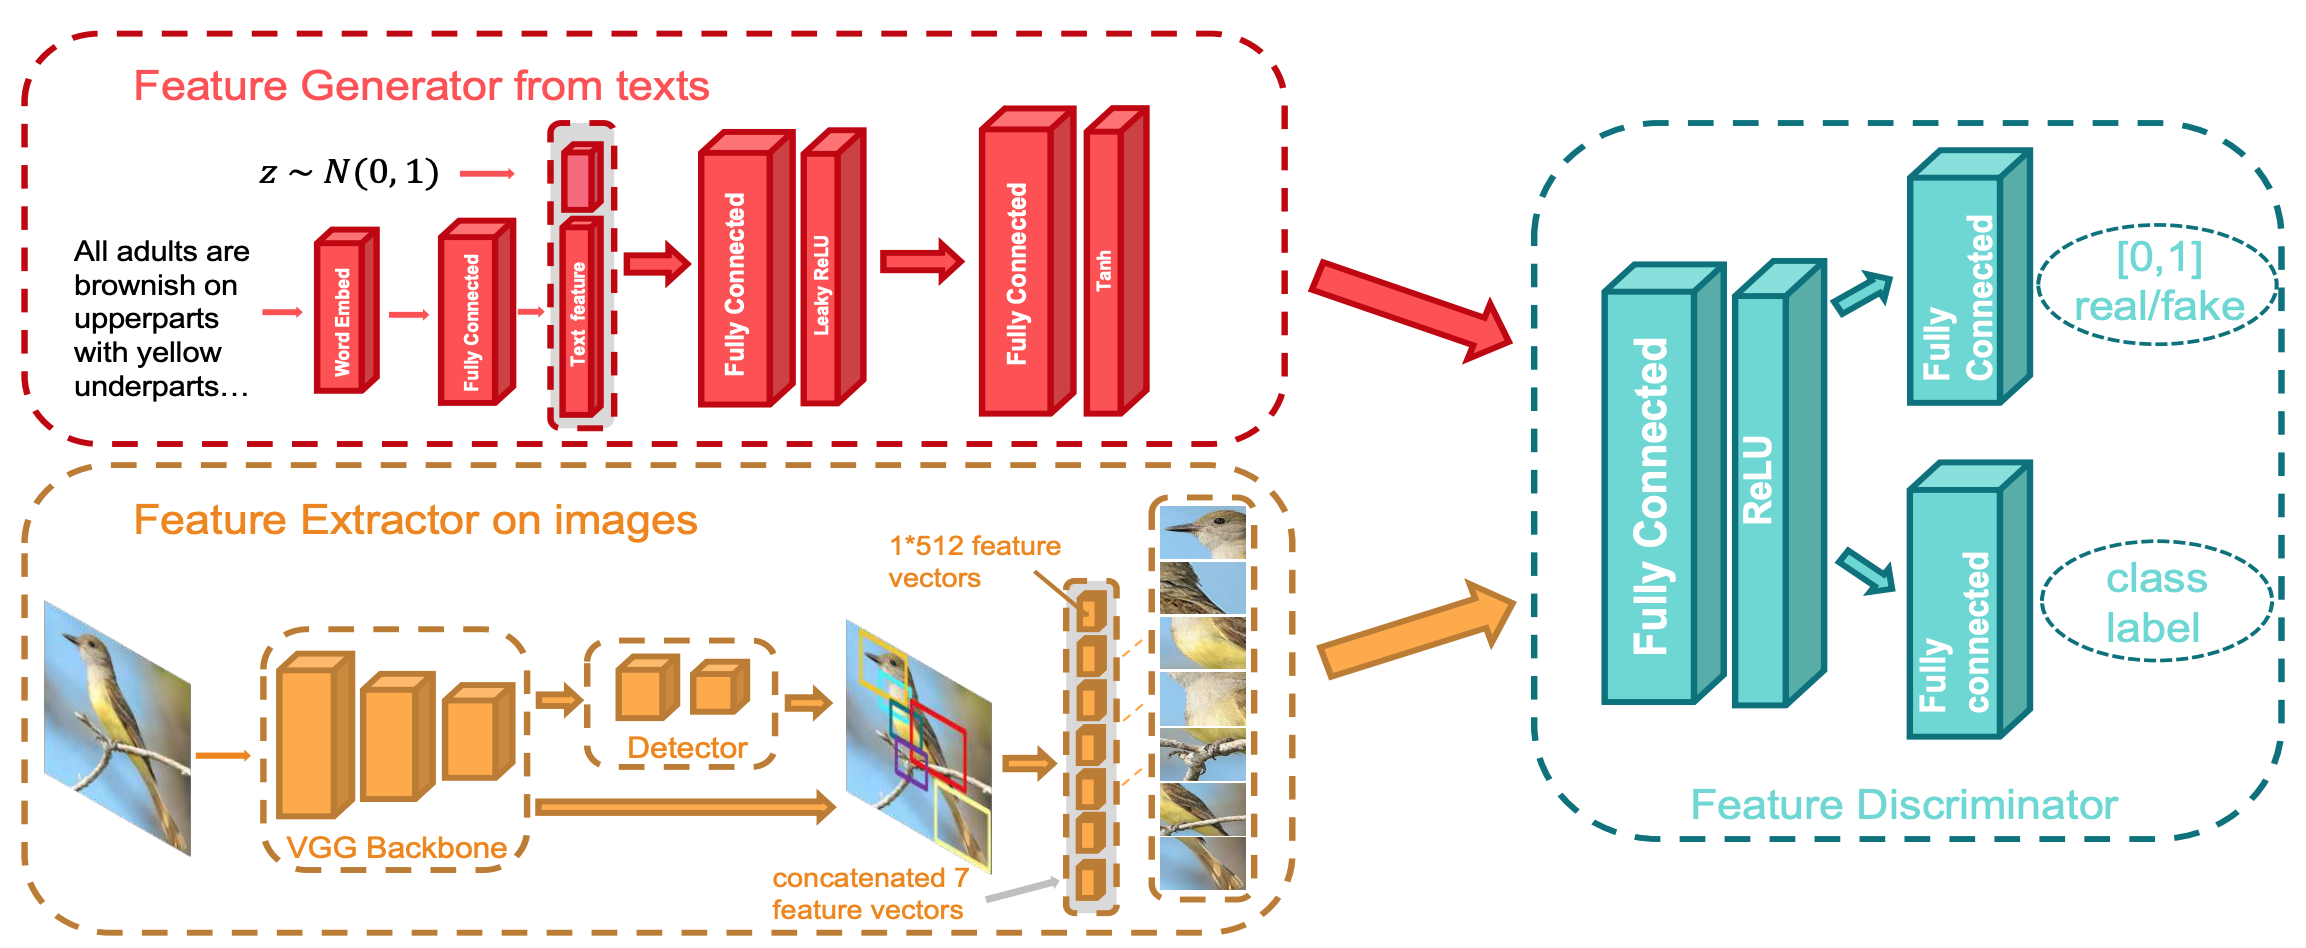
\includegraphics[width=\textwidth]{images/gazsl}
\end{frame}

\begin{frame}
    \frametitle{Generative Memory for Continual Learning \cite{MeRGAN}}
    
    \begin{itemize}
        \item For task $t$, train a conditional GAN model $(G_t, D_t)$ to save current dataset.
        \item Distill the knowledge of previous generator $G_{t-1}$ into $G_t$ so not to forget previous data.
        \item Train a classifier $C_t$ on top of $G_t$.
    \end{itemize}
    
    \vspace{0.5cm}
    \centering
    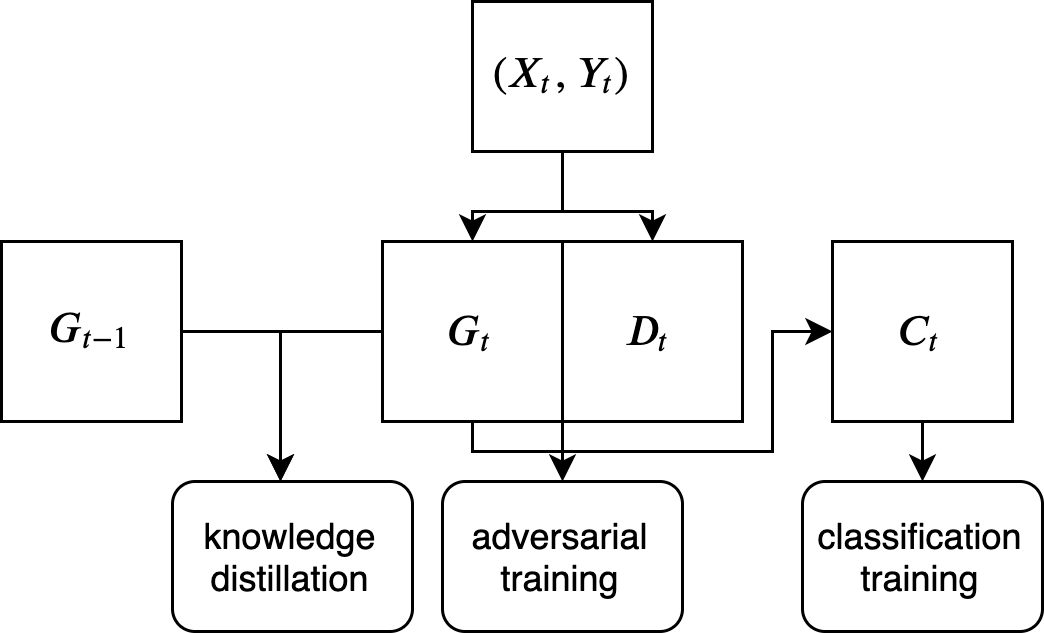
\includegraphics[width=0.6\textwidth]{images/genmem}
\end{frame}

\begin{frame}
    \frametitle{Zero-Shot Continual Learning}
    \begin{itemize}
        \item Merge two approaches: GAZSL + MeRGAN to improve future transfer.
        \item Since GAN model is difficult to train in high-scale image space, one can train it in either low-scale image space or latent space.
    \end{itemize}
    \vspace{0.5cm}
    \centering
    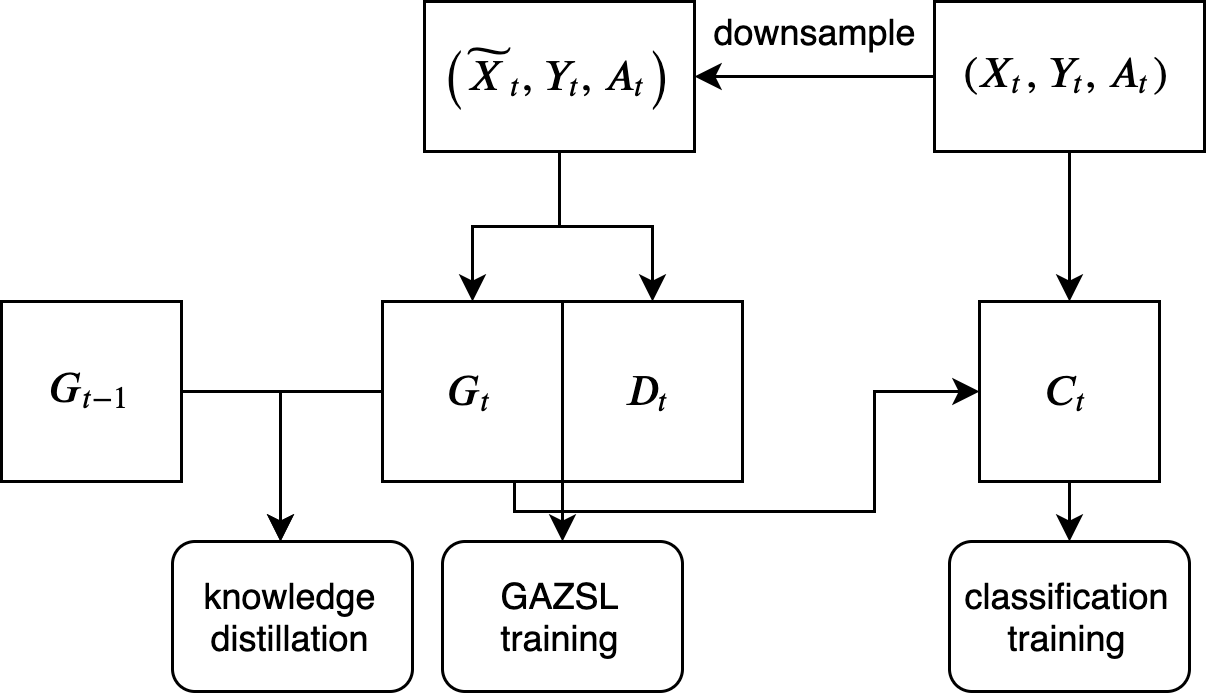
\includegraphics[width=0.7\textwidth]{images/latent-genmem}
\end{frame}

%\begin{frame}
%    \frametitle{Generalized experiment setup}
%    
%    Current CL setups are very segmented:
%    \begin{itemize}
%        \item Task boundaries: each task can include specific set of classes or we just have a changing distribution over classes.
%        \item Task identities: do we know which task an example is coming from?
%        \item Class-incremental learning: we are given several tasks, but evaluate on the joint class space.
%    \end{itemize}
%    
%    Simple generalization:
%    \begin{itemize}
%        \item 
%    \end{itemize}
%\end{frame}

\begin{frame}
    \frametitle{References}
    \printbibliography[heading=none]
\end{frame}
%\begin{frame}[noframenumbering,plain,allowframebreaks]{Literatur}
%    \printbibliography[heading=none]
%\end{frame}

\end{document}
